\label{sec:muroexe}


\begin{figure}[t]
	\centering
    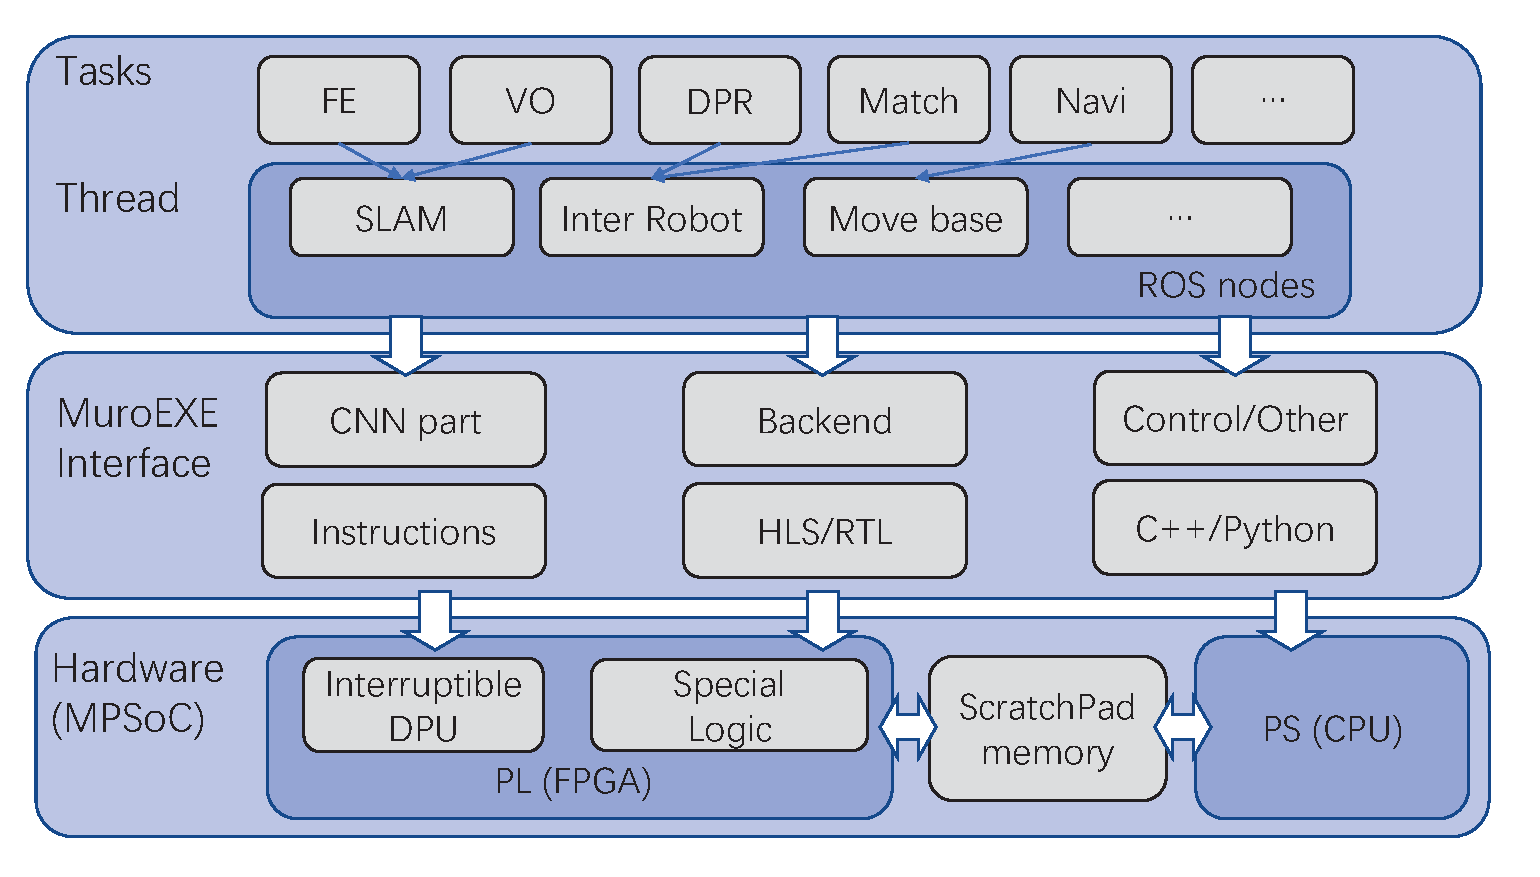
\includegraphics[width=0.99\linewidth]{fig/muroexe.eps}
    \caption{ Overview of the MUROEXE framework. Each ROS node is a separate thread. The CNNs in different ROS nodes are deployed onto the interruptible accelerator. The post-processing in the ROS nodes can accelerated by the RTL/HLS modules. The hardware modules for post-processing and the CNN accelerator share data through scrachpad memory. }
	\label{fig:muroexe}
\end{figure}

The design philosophy of MuroEXE is to use CNN as much as possible to accomplish various tasks on the robot. Because the CNN not only has advantages over traditional algorithms in accuracy, but also has uniform and regular computing mode. Therefore, a single instruction-driven CNN accelerator can speed up different tasks. The unified accelerator can reduce the use of hardware resources and make it easier to implement the robot computing system on embedded FPGA.

The framework MUROEXE is proposed to make the robotics community easy to use the FPGA accelerator. As the Robot Operating System (ROS) \cite{quigley2009ros} is a popular middleware fusing different modules from different developers, MUROEXE is designed for the multi-thread scheduling method in ROS, as illustrated in \Cref{fig:muroexe}.

In ROS, each function module is implemented as a node, and different nodes are executed in different CPU threads with asynchronous data sharing. Callback functions are used to process input data in ROS nodes. Once a ROS node subscribes to a data, and each time new data arrives, the corresponding callback function is executed.

Each ROS node does not care about the specific execution process of the hardware accelerator (we name the accelerator DNN Processing Unit, DPU). The software only needs to configure the priority of different tasks in different nodes ( the red parameter, priority, in line 13 in ROSExample 1 and line 9 in ROSExample 2). The hardware will automatically schedule the tasks according to the priority.

To eliminate the memory copy between CPU cores and CNN accelerators, we use low-latency ScratchPad memory \cite{Banakar2002Scratchpad} to directly feed the featuremaps extracted by CNN backbones to the post-processing modules. The blue lines in  ROSExample 1,2 illustrate the usage for the ScratchPad memory. Each shared date in DDR is initialized with two handlers: 1) a pointer (Ptr) for the CPU thread and 2) the physical address for the hardware modules. 

\begin{algorithm}[h]
    \caption{ Node for FE }
    \begin{algorithmic}[1]
        \State {\color{gray} // imagePtr, imageAddr, fmPtr, fmAddr, DPUtask, Bankendtask  is initialized by main and used in FEcallback.}
        \Function {FEcallback}{$ InputFrame $}
        \State {\color{gray} // Read and reshape the InputFrame. }
        \State {\color{blue} *imagePtr  $\gets$ *InputFrame }
        \State DPUtask.run()
        \State FEBackend.run()
        \EndFunction

        \Function {main}{$ $}
        \State {\color{gray} // Init ScratchPad Memory. Ptr is for CPU operations, Addr is for FPGA modules.}
        \State imagePtr, imageAddr = ScratchPad(FEinputsize)
        \State fmPtr, fmAddr = ScratchPad(FEfmsize)
        \State {\color{gray}// Config task0 in IAU of the accelerator (DPU).}
        \State DPUtask = FE\_DPUinit( {\color{red} priority=0 },{\color{blue}  inoffset=imageAddr,outoffset=fmAddr } ) 
        \State FEBackend = FEBackendinit({\color{blue}fmAddr, fmPtr});
        \State {\color{gray}// The node subscribes the inputframe, and use the FEcallback to process each inputframe.}
        \State Subscriber = Node.subscribe( InputFrame, FEcallback);
        \State {\color{gray}// Use spin to start the subscriber}
        \State Subscriber.spin();
        \EndFunction
    \end{algorithmic}
\end{algorithm}

\begin{algorithm}[h]
    \caption{ Node for PR }
    \begin{algorithmic}[1]
        \Function {PRcallback}{$ InputKeyFrame $}
        \State {\color{blue} *imagePtr  $\gets$ *InputKeyFrame }
        \State DPUtask.run()
        \State PRBackend.run()
        \EndFunction

        \Function {main}{$ $}
        \State imagePtr, imageAddr = ScratchPad(PRinputsize)
        \State fmPtr, fmAddr = ScratchPad(PRfmsize)
        \State DPUtask = PR\_DPUinit( {\color{red} priority=1 },{\color{blue} inoffset=imageAddr,outoffset=fmAddr } ) 
        \State PRBackend = PRBackendinit({\color{blue}fmAddr, fmPtr});
        \State Subscriber = Node.subscribe( InputKeyFrame, PRcallback);
        \State Subscriber.spin();
        \EndFunction
    \end{algorithmic}
\end{algorithm}
